\documentclass[12pt]{article}
\usepackage[paperwidth=36in,paperheight=24in,margin=0in]{geometry}
\usepackage{tikz,graphicx,xcolor,amsmath}
\pagestyle{empty}

% Editable color palette.
\definecolor{paper}{HTML}{E8E1CD}
\definecolor{header}{HTML}{79A9D8}
\definecolor{tan}{HTML}{C29D7F}
\definecolor{rose}{HTML}{BF7779}
\definecolor{blue}{HTML}{7EADDA}
\definecolor{violet}{HTML}{7D7CDB}
\definecolor{green}{HTML}{8FB88F}

\newcommand{\posterTitle}{Applied Spectral Graph Theory: Single-Cell Manifold Learning \& Network Connectivity}
\newcommand{\posterSubtitle}{Spring 2026 Independent Study: Anmol Singh Josan}

% This LaTeX file is an editable visual template. The compiled PDF in this
% folder was generated with build_spring_2026_poster_pdf.py because pdflatex
% was not available on PATH and Docker Desktop was not running.

\begin{document}
\pagecolor{paper}
\sffamily
\begin{tikzpicture}[x=1in,y=1in]
  \node[rounded corners=.14in,fill=header,minimum width=35.44in,minimum height=2.08in] at (18,-1.32) {};
  \node[align=center,text width=34in] at (18,-1.18) {
    {\fontsize{44}{48}\bfseries\selectfont \posterTitle}\\[.12in]
    {\fontsize{20}{22}\bfseries\selectfont \posterSubtitle}
  };

  % Use the Python builder for the current finished PDF. This TeX scaffold is
  % here so the poster can be converted to a full LaTeX workflow later.
  \node[anchor=north west,rounded corners=.12in,fill=tan,inner sep=.24in,text width=10.95in,minimum height=5.55in] at (.28,-2.58) {
    {\fontsize{33}{35}\bfseries\selectfont Introduction}\par\vspace{.1in}
    {\fontsize{16}{19}\selectfont Single-cell RNA sequencing creates high-dimensional data. Spectral graph theory turns cells into nodes, connects similar cells, and uses the graph Laplacian $L=D-A$ to find hidden communities.}
  };

  \node[anchor=north west,rounded corners=.12in,fill=violet,inner sep=.24in,text width=11.45in,minimum height=5.1in] at (12,-2.58) {
    {\fontsize{33}{35}\bfseries\selectfont The Fiedler Value \& Robustness}\par\vspace{.1in}
    {\fontsize{16}{19}\selectfont The second smallest Laplacian eigenvalue, $\lambda_2$, measures algebraic connectivity. If $\lambda_2>0$, the graph is connected; if it is close to zero, the network has a bottleneck.}
  };

  \node[anchor=north west,rounded corners=.12in,fill=tan,inner sep=.24in,text width=11.05in,minimum height=5.45in] at (24.2,-2.58) {
    {\fontsize{33}{35}\bfseries\selectfont Results \& Interpretation}\par\vspace{.1in}
    {\fontsize{16}{19}\selectfont The pipeline found five spectral communities and linked graph structure to clinical response hypotheses, including a T-cell response signal and myeloid resistance signal.}
  };

  \node[anchor=north west,rounded corners=.12in,fill=blue,inner sep=.24in,text width=11.45in,minimum height=9.02in] at (12,-7.88) {
    {\fontsize{33}{35}\bfseries\selectfont Case Study: Spectral Clustering}\par\vspace{.1in}
    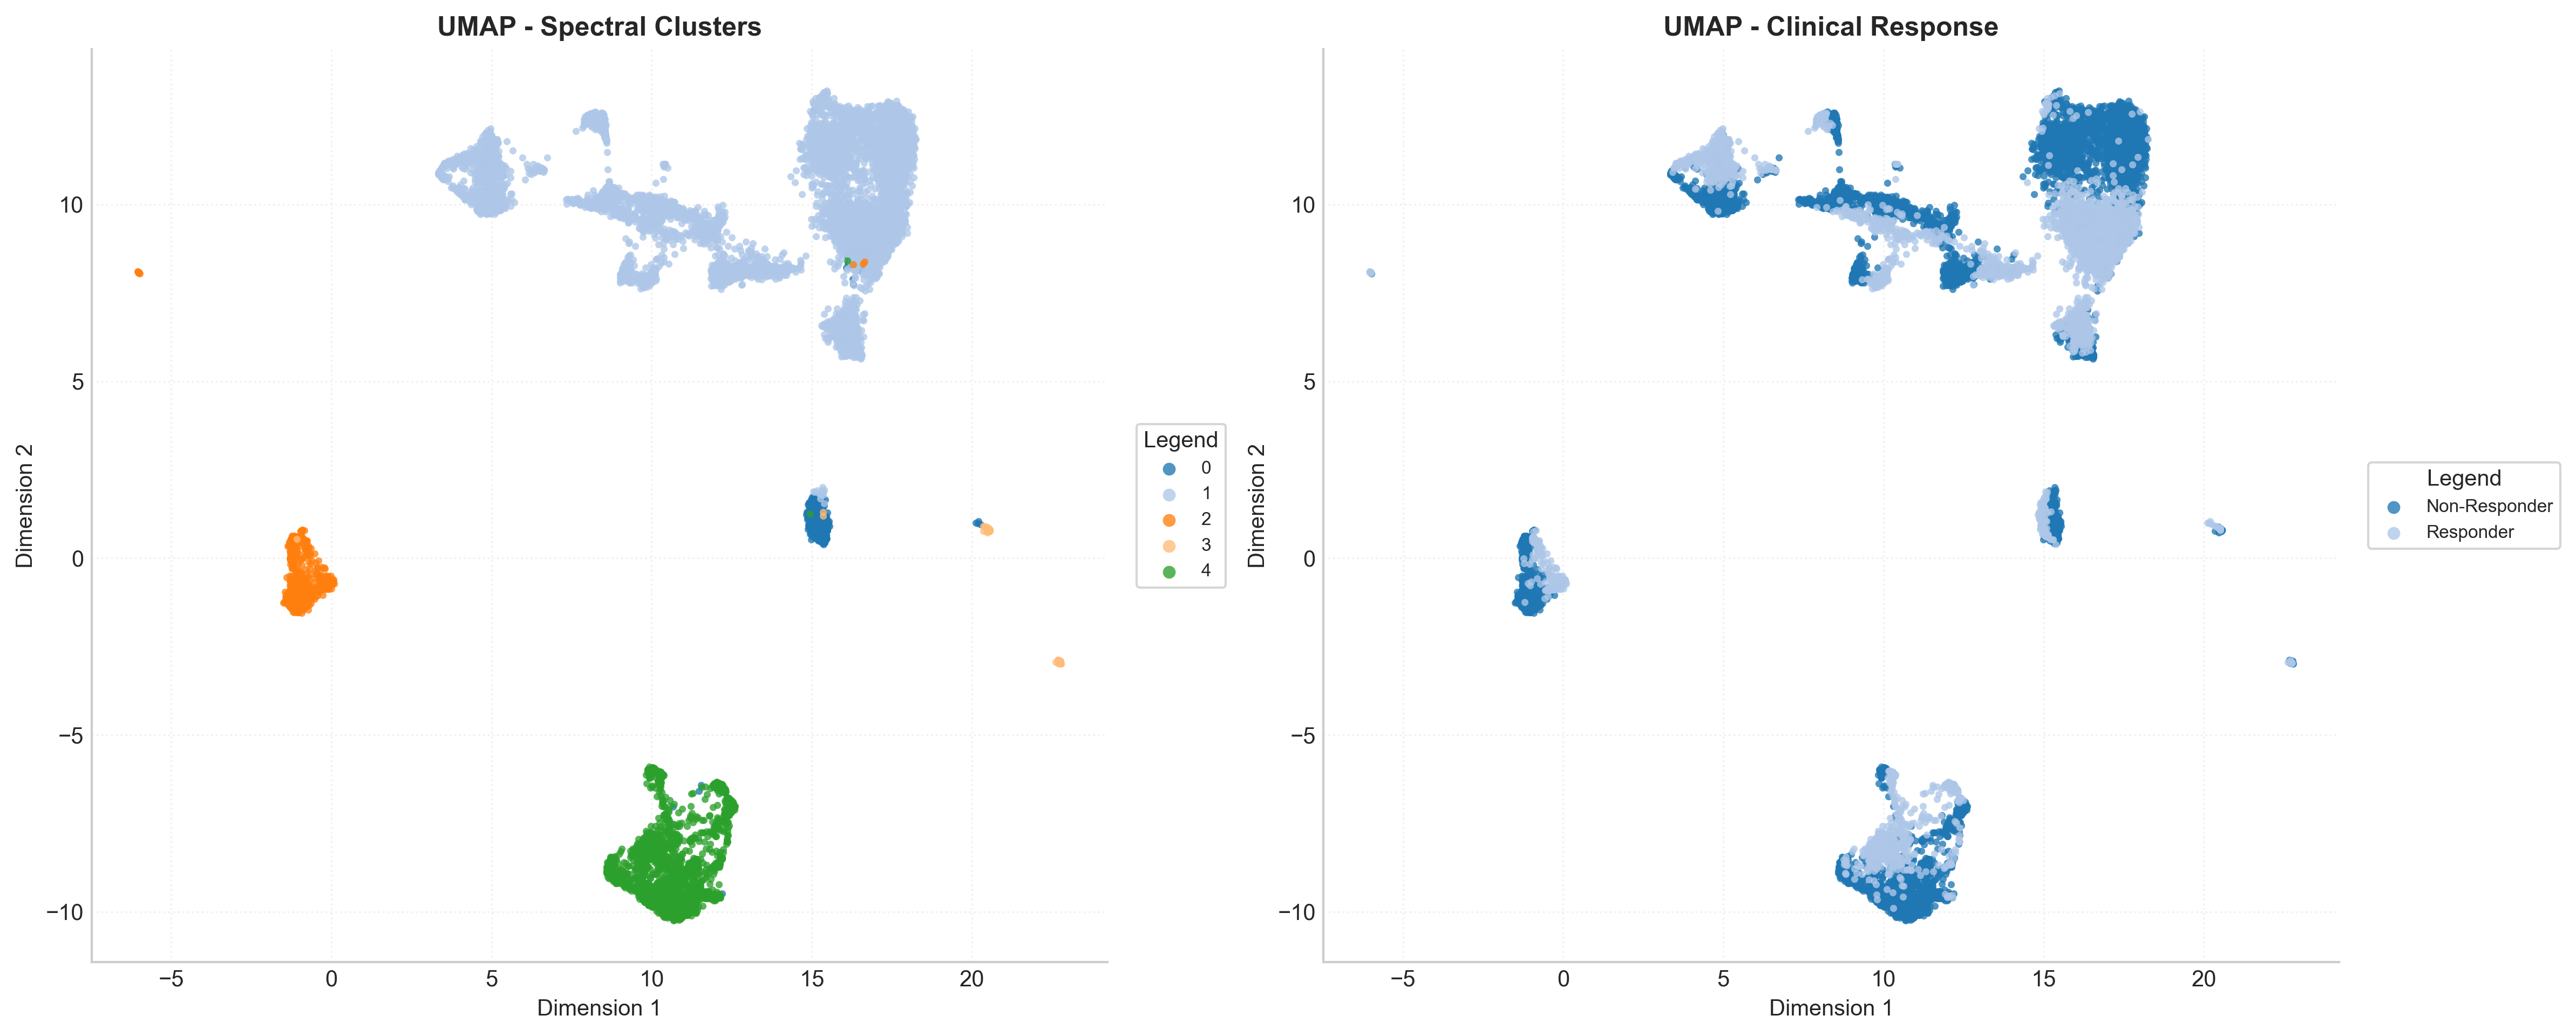
\includegraphics[width=11in,height=3in,keepaspectratio]{../plots/dots_umap_clusters_and_response.png}\par
    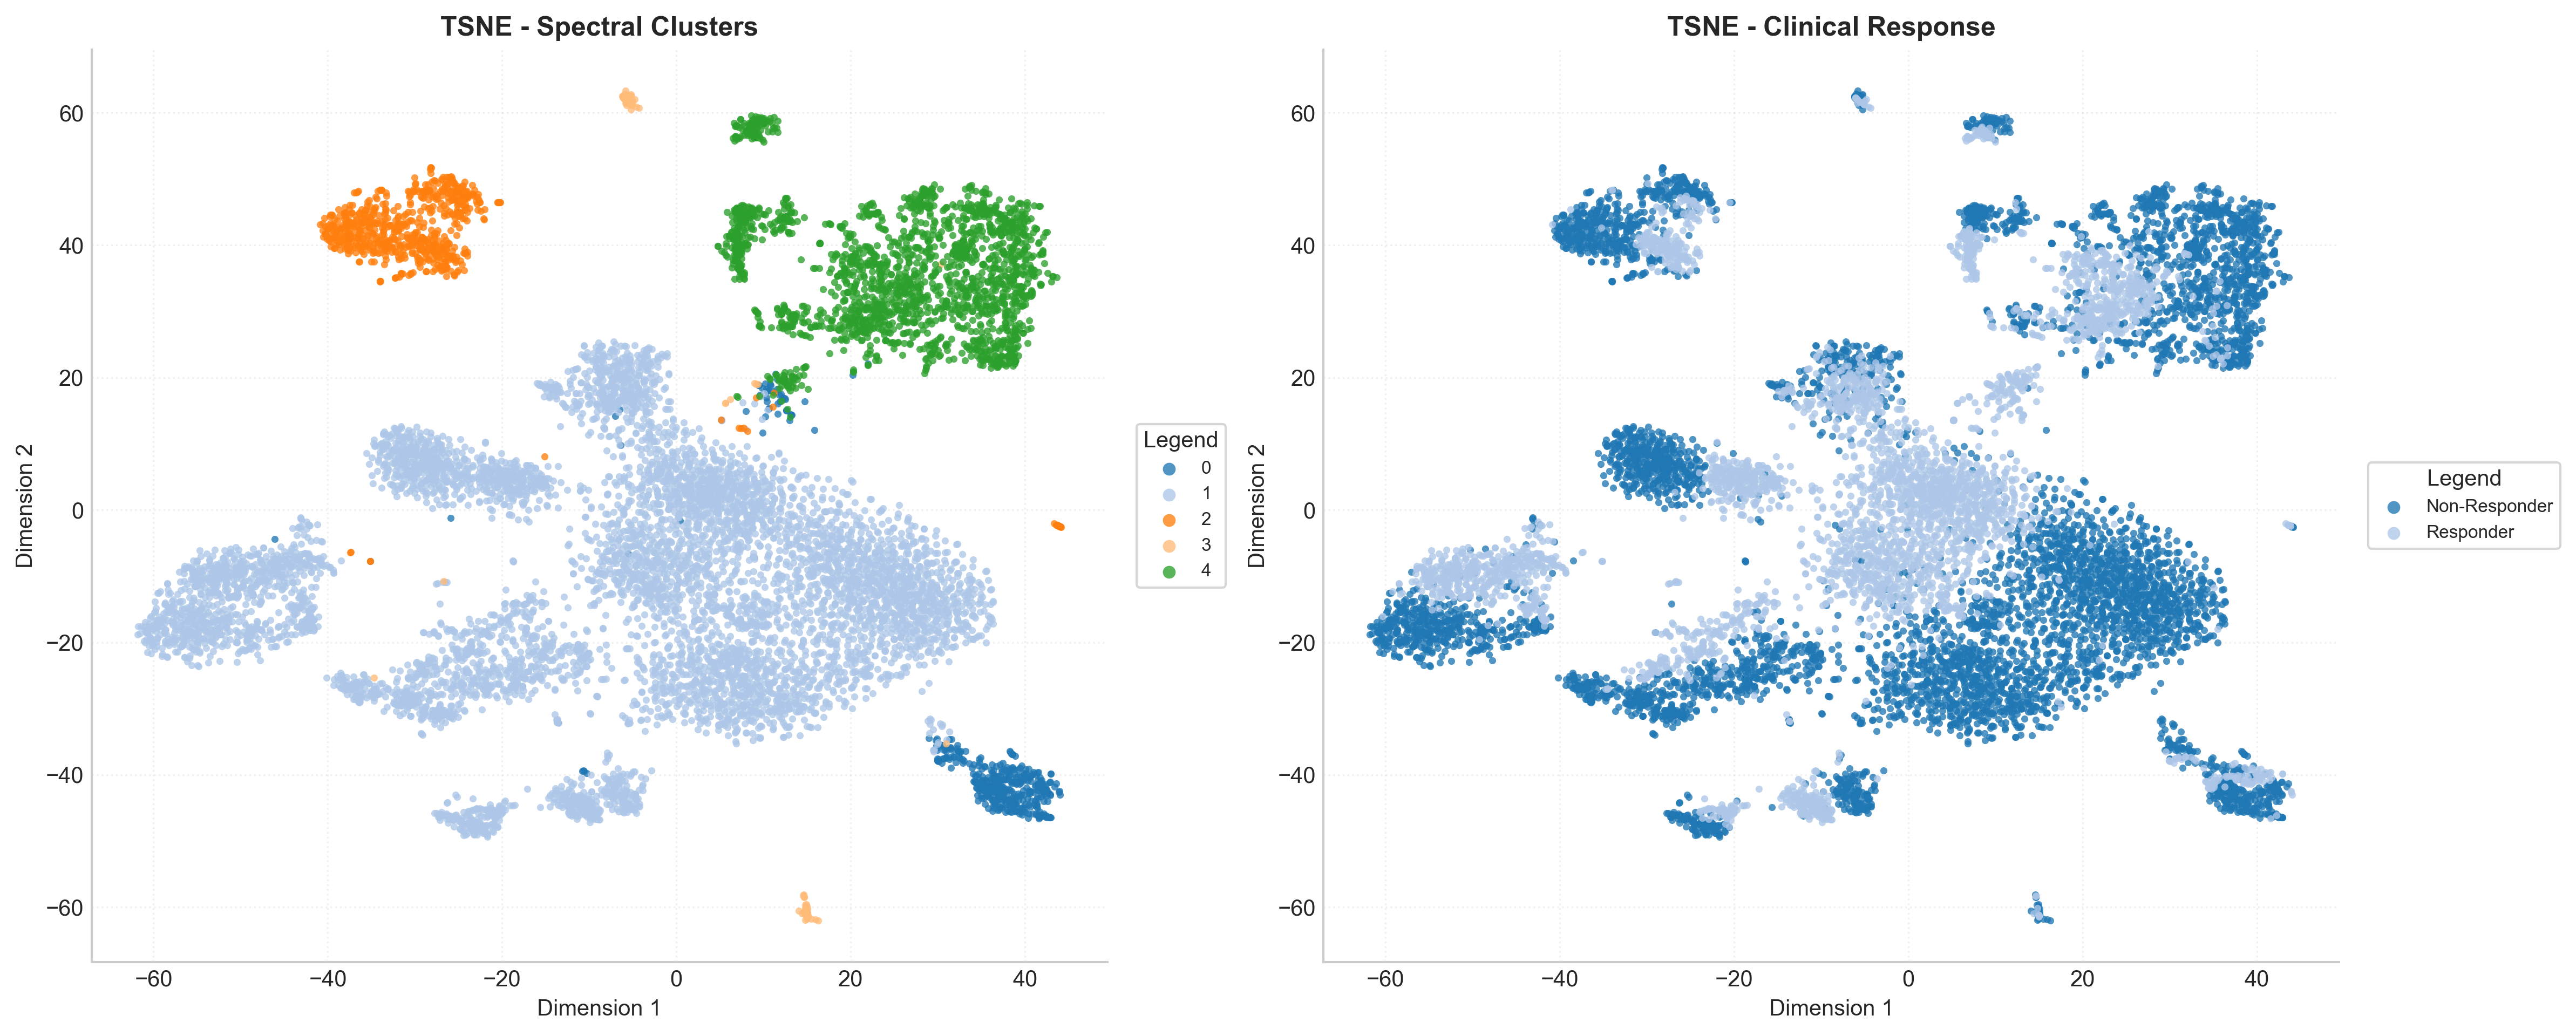
\includegraphics[width=11in,height=3in,keepaspectratio]{../plots/dots_tsne_clusters_and_response.png}
  };
\end{tikzpicture}
\end{document}
